\documentclass[a4paper, 14pt]{extarticle}
\usepackage{fontspec}
\setmainfont{CMU Serif}[Ligatures=TeX]
\setmonofont{CMU Typewriter Text}
\usepackage{polyglossia}
\setdefaultlanguage{russian}
\usepackage[left=1cm,right=1cm,top=2cm,bottom=2cm]{geometry}
%%% Дополнительная работа с математикой
\usepackage{amsfonts,amssymb,amsthm,mathtools} % AMS
\usepackage{amsmath}
\usepackage{icomma} % "Умная" запятая: $0,2$ --- число, $0, 2$ --- перечисление

\usepackage{mathrsfs} % Красивый матшрифт

%% Перенос знаков в формулах (по Львовскому)
\newcommand*{\hm}[1]{#1\nobreak\discretionary{}
  {\hbox{$\mathsurround=0pt #1$}}{}}

%%% Работа с картинками

\usepackage{graphicx}  % Для вставки рисунков
\graphicspath{ {grafs/} }
\setlength\fboxsep{3pt} % Отступ рамки \fbox{} от рисунка
\setlength\fboxrule{1pt} % Толщина линий рамки \fbox{}
\usepackage{wrapfig} % Обтекание рисунков и таблиц текстом

\usepackage[dvipsnames]{xcolor}
\usepackage{verbatim}
\usepackage{hyperref}
\usepackage{listings}

\lstdefinelanguage{JavaScript}{
  keywords={let, typeof, new, true, false, catch, function, return, null, catch, switch, var, if, in, while, do, else, case, break},
  keywordstyle=\color{blue}\bfseries,
  ndkeywords={class, export, boolean, throw, implements, import, this},
  ndkeywordstyle=\color{darkgray}\bfseries,
  identifierstyle=\color{black},
  sensitive=false,
  comment=[l]{//},
  morecomment=[s]{/*}{*/},
  commentstyle=\color{purple}\ttfamily,
  stringstyle=\color{red}\ttfamily,
  morestring=[b]',
  morestring=[b]"
}

\lstset{
  language=JavaScript,
  extendedchars=true,
  basicstyle=\footnotesize\ttfamily,
  showstringspaces=false,
  breakatwhitespace=true,
  showspaces=false,
  numbers=left,
  numberstyle=\footnotesize,
  numbersep=9pt,
  tabsize=2,
  keepspaces=true,
  breaklines=true,
  showtabs=false,
  captionpos=b
  escapechar =| ,
  frame=single ,
  commentstyle=\itshape ,
  stringstyle =\bfseries
}

\newcommand*{\function}[2]{\texttt{\textcolor{Red}{function} \textcolor{Purple}{#1}(#2)}}

\newcommand*{\prototype}[3]{\texttt{\textcolor{Orange}{#1}.\textcolor{Blue}{prototype}.\textcolor{Purple}{#2} = \textcolor{Red}{function}(#3)}}

\usepackage{titlesec}

\setcounter{secnumdepth}{4}

\titleformat{\paragraph}
{\normalfont\normalsize\bfseries}{\theparagraph}{1em}{}
\titlespacing*{\paragraph}
{0pt}{3.25ex plus 1ex minus .2ex}{1.5ex plus .2ex}

\usepackage{multicol}
\setlength{\columnsep}{1cm}

\begin{document}


\begin{center}
	\hfill \break
	\large{МИНОБРНАУКИ РОССИИ}\\
	\footnotesize{ФЕДЕРАЛЬНОЕ ГОСУДАРСТВЕННОЕ БЮДЖЕТНОЕ ОБРАЗОВАТЕЛЬНОЕ УЧРЕЖДЕНИЕ}\\
	\footnotesize{ВЫСШЕГО ПРОФЕССИОНАЛЬНОГО ОБРАЗОВАНИЯ}\\
	\small{\textbf{«ВОРОНЕЖСКИЙ ГОСУДАРСТВЕННЫЙ УНИВЕРСИТЕТ»}}\\
	\hfill \break
	\normalsize{Математический факультет}\\
	\hfill \break
	\normalsize{Кафедра теории функций и геометрии}\\
	\hfill\break
	\hfill \break
	\hfill \break
	\hfill \break
	\large{Программная реализация (на языке JavaScript) алгоритмов генерации ФОС по математике 2023}\\
	\hfill \break
	\hfill \break
	\hfill \break\
	\hfill \break
	\hfill \break
	\normalsize{Курсовая работа\\
		\hfill \break
		Направление  010501 Фундаментальные математика и механика\\

		\hfill \break
	}\\
	\hfill \break
	\hfill \break
\end{center}
\hfill \break

\normalsize{
	\begin{tabular}{cccc}
		Зав.кафедрой & \underline{\hspace{3cm}} & д.физ.-мат.н.,  проф. & Е.М. Семёнов    \\\\
		Обучающийся  & \underline{\hspace{3cm}} &                       & А.С. Суматохина \\\\
		Руководитель & \underline{\hspace{3cm}} & д.физ.-мат.н.,  проф. & Е.М. Семёнов    \\\\
	\end{tabular}
}\\
\hfill \break
\hfill \break
\begin{center} Воронеж 2023 \end{center}
\thispagestyle{empty} % выключаем отображение номера для этой страницы

% КОНЕЦ ТИТУЛЬНОГО ЛИСТА


\tableofcontents


\section*{Введение}
\addcontentsline{toc}{section}{Введение}
Единый государственный экзамен (ЕГЭ)~ — централизованно проводимый в Российской
Федерации экзамен в средних учебных заведениях — школах, лицеях и гимназиях,
форма проведения ГИА(Государственный Итоговая Аттестация) по образовательным программам среднего общего образования.
Служит одновременно выпускным экзаменом из школы и вступительным экзаменом в вузы.

За два года подготовки к ЕГЭ школьники сталкиваются с дефицитом заданий для подготовки.
А учителя со списыванием ответов при решении задач экзамена учениками.
Также в конце 2021 года в список заданий ЕГЭ были добавлены новые задания под номером 9,
количество которых для прорешивания очень мало. Помимо перечисленного существуют задания, на решение которых требуется менее минуты, а их составление вручную занимает несоразмерно много времени.
Проект «Час ЕГЭ» позволяет решить все эти проблемы.

«Час ЕГЭ» — компьютерный образовательный проект, разрабатываемый при математическом
факультете ВГУ в рамках «OpenSource кластера» и предназначенный для помощи учащимся
старших классов подготовиться к тестовой части единого государственного экзамена.
%%ссылочки на доклады
Задания в «Час ЕГЭ» генерируются случайным образом по специализированным алгоритмам,
называемых шаблонами, каждый из которых
охватывает множество вариантов соответствующей ему задачи. Для
пользователей
предназначены четыре оболочки (режима работы): «Случайное задание», «Тесты на печать»,
«Полный тест» и «Мини-интеграция».
«Час ЕГЭ» является полностью открытым (код находится под лицензией GNU GPL 3.0)
и бесплатным.
В настоящее время в проекте полностью реализованы тесты по математике с кратким
ответом (бывшая «часть В»).~\cite{fipi}
Планируется с течением времени включить в проект тесты по другим предметам школьной
программы.

«Мини-интеграция» — это форма сотрудничества с образовательными интернет-ресурсами,
при которой учебно-методический материал на странице ресурса дополняется виджетами
тренажера с заданиями, соответствующими теме статьи, для возможности практического
применения полученных знаний.
В настоящее время достигнуто сотрудничество с двумя образовательными ресурсами: ege-ok.ru
и matematikalegko.ru.



%%Программная реализация (на языке Javascript) алгоритмов
%% генерации фонда оценочных средств по математике
\section{Глава первая}
\subsection{Реализация алгоритмов на базе проекта Час ЕГЭ}
Как было уже сказано ранее, генерация заданий происходит при помощи шаблонов.
Программная реализация на языке JavaScript обеспечивает генерацию текстового задания,
графической на основе canvas
\footnote{HTML элемента, использующегося для рисования графики средствами языков программирования и алгоритма решения задачи} в случае необходимости,
ответа и иногда подробного решения.

Алгоритм написания простого шаблона~\cite{chasi} на основе номера 109083 Открытого Банка Заданий ЕГЭ~\cite{fipi}:
\begin{enumerate}
	\item Выбираем задание из Открытого Банка Заданий ЕГЭ и копируем его текст.
	\item Добавляем ответ в поле answers (по умолчанию 0).
	      \lstinputlisting{code/listing_1.1.js}
	\item Инициализируем всех необходимые переменные для задачи (вес, проценты и так далее).
	      Присваиваем им значения при помощи функции \hyperlink{sluchch}{sluchch()} или
	      \hyperlink{slKrome}{slKrome()} (см. главу \ref{2sect}). Для хранения ответа создаём отдельную переменную.
	      \lstinputlisting{code/listing_1.2.js}
	\item Заменяем все числа в тексте на переменные (при помощи +'\cdot'+).
	\item Обособляем слова, которые не влияют на условия задачи. Это могут быть
	      имена, профессии, транспорт и т.п.
	\item Создаём переменные, которые будет отвечать за выбранные в прошлом пункте
	      слова, и заменяем слова на переменные в тексте задачи.
	      Выбираем их значения из массивов при помощи \hyperlink{iz}{iz()} (см. главу \ref{2sect}).
	\item Иногда в задании выбранные слова используются в разных падежах.
	      Для этого в проекте существует лексический модуль.
	      Используем на склоняемых словах функцию \hyperlink{sklonlxkand}{sklonlxkand()}.
	      Теперь необходимо указать падеж слов в задании.
	      Также при необходимости заглавной буквы в слове используем
	      \hyperlink{toZagl}{toZagl()} (см. главу \ref{2sect}).
	\item Если в тексте задачи присутствуют слова, зависимые от числительных,
	      к ним применяется функция \hyperlink{chislitlx}{chislitlx()} (см. главу \ref{2sect}).
	      \lstinputlisting{code/listing_1.3.js}
\end{enumerate}

Но не все задачи решаются при помощи линейного алгоритма. Тогда в коде шаблона
используется слишком много циклов с постусловиями (или предусловиями)
Для таких случаев в проекте существует функция retryWhileUndefined(), которое
будет запускать программу до тех пор, пока случайные переменные не будут удовлетворять всем условиям.
Перезапуск осуществляется посредством постановки условий с последующим return.
Рассмотрим такой пример.

\textbf{Алгоритм написания шаблона с изображением графика прямой:}
\begin{enumerate}
	\item Для отображения рисунка необходимо вызвать функцию chas2.task.modifiers.
	      addCanvasIllustration(), которой передаются высота и ширина изображения и функция отрисовки.
	      \lstinputlisting{code/listing_2.1.js}
	\item Пусть наша прямая проходит через две точки $(x_1,y_1)$ и $(x_2,y_2)$. Инициализируем их координаты случайными целыми числами. Теперь через них выразим коэффициенты уравнения прямой $y=kx+b$.
	      Для дальнейшего вычисления точек прямой напишем вспомогательную функцию $f(x)$.
	      \lstinputlisting{code/listing_2.2.js}

	\item Для того, чтобы уравнения нашей прямой можно было восстановить по рисунку, необходимо и достаточно,
	      чтобы были видны две её точки. Для поиска таких точек используем функцию \hyperlink{intPoints}{intPoints()} (см. главу \ref{2sect}).
	      \lstinputlisting{code/listing_2.3.js}
	\item Приступим к изображению графика. Инициализируем переменную paint1 как функцию function(ct). Внутри неё зададим высоту и ширину графика в пикселях.
	      Изображаем координатную плоскость функцией \hyperlink{drawCoordPlane}{drawCoordPlane()} и сам график функцией
	      \hyperlink{graph9AdrawFunction}{graph9AdrawFunction()}. А также отметим две целые точки посредством \hyperlink{graph9AmarkCircles}{graph9AmarkCircles()} (см. главу \ref{2sect}).
	      \vspace{\baselineskip}

	      \lstinputlisting{code/listing_2.4.js}
\end{enumerate}

\textbf{Алгоритм написания шаблона с изображением графика производной:}

\begin{enumerate}
	\item Для отображения рисунка необходимо вызвать функцию chas2.task.modifiers.
	      addCanvasIllustration(), которой передаются высота и ширина изображения и функция отрисовки.\\
	      \\
	      \lstinputlisting{code/listing_3.1.js}
	\item Определяем область определения будущей функции и заполняем два массива, где будут находиться координаты точек, через которые будет проходить график функции.
	      Строим график по точкам при помощи библиотеки \texttt{cubic-spline}.
	      \lstinputlisting{code/listing_3.2.js}
	\item Находим экстремумы функции, промежутки её возрастания и убывания.
	      \lstinputlisting{code/listing_3.3.js}
	\item Отрисовываем график, определяем задание.
	      \lstinputlisting{code/listing_3.4.js}

\end{enumerate}

\subsection{Преимущества программной генерации заданий}
На примере двух предыдущих задач были явно показано превосходство шаблонов над заданиями из Открытого Банка Заданий, а именно:
\begin{enumerate}
	\item Большое количество разнообразных задач одного типа.
	\item Простота и скорость написания шаблонов.
	\item Невозможность нахождения учащимися ответов на задачи.
\end{enumerate}



\section{Глава вторая}\label{2sect}
\subsection{Функции, используемые в проекте}
За 9 лет работы над проектом «Час ЕГЭ» была разработан нестандартная библиотека для упрощения многих задач. Далее представлены наиболее используемые функции из неё.

\subsubsection*{Работа с массивами}

\paragraph*{Многочлены}

Элементы одномерного массива Array --- коэффициенты, стоящие в порядке возрастания степеней.

\prototype{Array}{mn\_proizv}{}

Находит производную от многочлена.

\prototype{Array}{mn\_vychisl}{}

Находит корни многочлена.

\prototype{Array}{mn\_txt}{}

TeX-представление многочлена.%%%???

\prototype{Array}{mn\_pervoobr}{}

Находит первообразную от многочлена.%%TODO: в чёр разница то??

\prototype{Array}{mn\_txtmas}{}

TeX-представление многочлена.

\prototype{Array}{mt\_pryam}{}

Возвращает коэффициенты $a$ и $b$ прямой $y=ax+b$, проходящей через две первые точки.

\paragraph*{Вспомогательные функции для массивов}

\prototype{Array}{shuffle}{b}

Перемешивает массив случайным образом. Если b, то ещё и рекурсивно на один уровень.

\hypertarget{iz}{\prototype{Array}{iz}{p1}}

Если p1 опущено, возвращает случайный элемент массива, иначе массив p1 неповторяющихся элементов массива.

\paragraph*{Матрицы}

\function{multiplyMatrix}{A,B}

Умножает матрицу A на B, возвращает результат в матрице C.

\function{Determinant}{A}

Возвращает определитель матрицы A.

\function{MatrixCofactor}{i,j,A}

Возвращает алгебраическое дополнение матрицы A.

\function{AdjugateMatrix}{A}

Возвращает союзную(присоединенную) матрицу.

\function{rang\_mat}{А}

Возвращает ранг матрицы A.

\function{InverseMatrix}{B}

Возвращает обратную  к B матрицу.

\function{generateMatrix}{stroki,stolbcy,min,max,p1}

Генерирует матрицу из случайных чисел.

\subsubsection*{Работа с числами}

\hypertarget{chislitlx}{\prototype{Number}{chislitlx}{p1,p2}}

Возвращает строку, состоящую из данного числа и подходящего падежа слова p1, при этом
полученное словосочетанию стоит в падеже p2 (если не указан - именительный).

\prototype{Number}{pow}{n}

Возвращает число в степени n.

\prototype{Number}{sqrt}{n}

Возвращает квадратный корень из числа.

\prototype{Number}{sqr}{}

Возвращает квадрат числа.

\prototype{Number}{abs}{}

Возвращает модуль числа.

\prototype{Number}{floor}{}

Возвращает число, округленное до целого в меньшую сторону.

\prototype{Number}{ceil}{}

Возвращает число, округленное до целого в большую сторону.

\prototype{Number}{pm}{}

Случайным образом возвращает число или ему противоположное.

\prototype{Number}{ts}{}
%%зачем? и пример
Приводит число к стандартному виду (с десятичной запятой и не более чем 10 знаками после неё).
Необходимо для отсечения ложной точности.

Пример:%%0.1+0.2
\begin{lstlisting}[frame=none]
let number1=0.7+0.1;
let number2=(0.7+0.1).ts()
\end{lstlisting}
\fbox{
	\parbox{10cm}{
		$number1=0.7999999999999999$

		$number2=0,8$
	}}



\prototype{Number}{texfracpi}{p1}

Возвращает TeX-представление дроби, у которой в числителе данное число, умноженное на $\pi$, а в знаменателе $p1$.
Случай $p1=1$ учитывается.

\prototype{Number}{texsqrt}{p1,p2}

TeX-представление корня из данного числа.
Если данное число - полный квадрат, то корень из числа.
Если p1, то из-под корня будут вынесены возможные множители.
Если p1, p2 и из-под корня выносится единица, то она будет опущена.

\prototype{Number}{isZ}{}

Возвращает true, если число n целое.

\prototype{Number}{isPolnKvadr}{}

Возвращает true, если число является полным квадратом.

\subsection{Работа со строками}

\hypertarget{toZagl}{\prototype{Number}{toZagl}{}}

Возвращает исходную строку с первой заглавной буквой.

\prototype{Number}{esli}{}

Возвращает данную строку, если p1, и пустую в противном случае.

\prototype{Number}{plusminus}{}

Возвращает упрощенное выражение, вставляя между числами необходимые знаки и убирая нулевые.

\subsubsection*{Работа с canvas}

\prototype{CanvasRenderingContext2D}{drawLine}{x1,y1,x2,y2}

Рисует линию из точки (x1,y1) в (x2,y2).

\prototype{CanvasRenderingContext2D}{fillKrug}{x,y,r}

Рисует круг с центром в (x,y) и радиусом r.

\prototype{CanvasRenderingContext2D}{drawArrow\newline}{x1, y1, x2, y2, arrowType}%%TODO Узнать зачем arrowType

Рисует стрелку из точки (x1,y1) в (x2,y2).

\hypertarget{drawCoordPlane}{
	\prototype{CanvasRenderingContext2D}{drawCoordPlane\newline}{w, h, kl, text, mash}}

Рисует координатную плоскость. w и h  \--- её размеры, kl \--- объект с полями hor и ver (высота и ширина клетки), text \-- объект с полями x1 и y1(единичные отрезки типа string), sh1 и sh2 (шрифты для x1, y1, по умолчанию 12px) и mash - масштаб изображения (по умолчанию равно 1).

\prototype{CanvasRenderingContext2D}{setkaVer2\newline}{h, w, hor, ver, mash}

Рисует прямоугольную сетку. w и h  \--- её размеры, hor и ver \--- высота и ширина клетки, mash - масштаб (по умолчанию равно 1).

\hypertarget{graph9AmarkCircles}{\function{graph9AmarkCircles}{ct, XY, maxQuantity, radius}}

Изображает не более maxQuantity точек в координатах из двумерно массива XY в виде кругов радиусом radius.
%%Переписать!

\hypertarget{graph9AdrawFunction}{\function{graph9AdrawFunction}{ct,f, o}}

Рисует график f(x). Границы отображения задаются объектом o с полями maxX, maxY, minX, minY.

\subsubsection*{Вспомогательные функции}

\hypertarget{sluchch}{\function{sluchch}{n,k,s}}

Возвращает случайное число от n до k с шагом s (по умолчанию 1).
Эта функция используется настолько часто, что для неё была придумана сокращённая форма sl().

\hypertarget{slKrome}{\function{slKrome}{a,p1,p2,p3}}

Возвращает случайное число, кроме a. Если a \--- массив, то не содержащееся в нём; если число или строка, то не равное ему; Если функция, принимающая параметр - то не удовлетворяющее ей.

\function{sluchDel}{a}

Возвращает случайный делитель числа a.

\function{sluchiz}{a,n}

Возвращает массив из n случайных не повторяющихся элементов массива a.

\function{slLetter}{b}

Возвращает случайную букву английского алфавита.%%зачем b?

\hypertarget{intPoints}{\function{intPoints}{f,o}}

Возвращает двумерный массив из всех целых точек графика f(x). Границы нахождения точек задаются объектом o с полями maxX, maxY, minX, minY.

\subsection{Вклад автора в расширение каталога}

\subsubsection*{Задание №109083}
\lstinputlisting{code/ex_109083.js}
Примеры генерируемых задач:

\vspace{\baselineskip}
\fbox{%
	\parbox{17cm}{%
		При сушке абрикоса получается курага. Сколько килограммов абрикоса
		потребуется для получения 66 килограммов кураги, если абрикос содержит
		90\% воды, а курага содержит 20\% воды?}%
}
\vspace{\baselineskip}

\fbox{%
	\parbox{17cm}{%
		При сушке дыни получается сухофрукт. Сколько килограммов дыни потребуется
		для получения 73 килограммов сухофрукта, если дыня содержит 88\% воды, а
		сухофрукт содержит 7\% воды?}%
}
\vspace{\baselineskip}

\fbox{%
	\parbox{17cm}{%
		При сушке винограда получается изюм. Сколько килограммов винограда
		потребуется для получения 70 килограммов изюма, если виноград содержит
		81\% воды, а изюм содержит 5\% воды?}%
}
\vspace{\baselineskip}
\subsubsection*{Задание №99621}
\lstinputlisting{code/ex_99621.js}

Примеры генерируемых задач:

\vspace{\baselineskip}
\fbox{%
	\parbox{17cm}{%
		Максим и Арина выполняют одинаковую экзаменационную работу. Арина решает
		за час 7 заданий работы, а Максим 8. Они одновременно начали выполнять
		задания, и Арина закончила работу позже Максима на 60 минут. Сколько заданий
		содержит работа?}%
}

\vspace{\baselineskip}
\fbox{%
	\parbox{17cm}{%
		Матвей и Ирма выполняют одинаковую контрольную работу. Ирма решает за час
		9 примеров работы, а Матвей 10. Они одновременно начали решать примеры,
		и Ирма закончила работу позже Матвея на 20 минут. Сколько примеров содержит
		работа?}%
}

\vspace{\baselineskip}
\fbox{%
	\parbox{17cm}{%
		Коля и Женя выполняют одинаковый тест. Женя отвечает за час на 9 вопросов
		теста, а Коля 10. Они одновременно начали отвечать на вопросы, и Женя
		закончила тест позже Коли на 40 минут. Сколько вопросов содержит тест?}%
}
\vspace{\baselineskip}
\subsubsection*{Задание №26775}
\lstinputlisting{code/ex_26775.js}
Примеры генерируемых задач:

\vspace{\baselineskip}
\fbox{%
	\parbox{17cm}{%
		Найдите $\ctg H$, если $\sin H=-\sqrt{\frac{9}{738}}$ и $H\in(37π;75π2)$.

		Найдём $\cos H\sqrt{1-(-\sqrt{\frac{9}{738}})^2=-\sqrt{\frac{729}{738}}}$(Угол H принадлежит
		III четверти - $\cos H<0$). Тогда $\ctg H=\sqrt{\frac{729}{9}}=9$}
}

\vspace{\baselineskip}
\fbox{%
	\parbox{17cm}{%
		Найдите $\tg M$, если $\cos M=\sqrt{\frac{4}{260}}$ и $M\in(\frac{101}{2}π;51π)$.

		Найдём $\sin M=\sqrt{1-(-\sqrt{\frac{9}{738}})^2=-\sqrt{\frac{729}{738}}}$(Угол  M принадлежит
		VI четверти - $sin M<0$). Тогда $\tg  M=\sqrt{\frac{256}{4}}=-8$}
}

\vspace{\baselineskip}
\fbox{%
	\parbox{17cm}{%
		Найдите $\tg Q$, если $\cos Q=-\sqrt{\frac{9}{153}}$ и $Q\in(\frac{171}{2}π;86π)$.

		Найдём $\sin = Q\sqrt{1-(-\sqrt{\frac{9}{153}})^2=\sqrt{\frac{144}{153}}}$(Угол  Q принадлежит
		VI четверти - $sin Q>0$). Тогда $\tg  Q=\sqrt{\frac{144}{9}}=-4$}
}
\subsubsection*{Задание №26771}
\lstinputlisting{code/ex_26771.js}
Примеры генерируемых задач:

\vspace{\baselineskip}
\fbox{%
	\parbox{17cm}{%
		Найдите значение выражения $-72\tg201^{\circ}\cdot\tg249^{\circ}$.

		По формуле приведения $\tg249^{\circ}=\tg(450^{\circ}-249^{\circ})=\ctg201^{\circ}$.
		Тогда $-72\tg 201^{\circ}\cdot\ctg 201^{\circ}=-72$}}

\vspace{\baselineskip}
\fbox{%
\parbox{17cm}{%
Найдите значение выражения $-58\tg400^{\circ}\cdot \tg410^{\circ}$.

По формуле приведения $\tg410^{\circ}=\tg(810^{\circ}-410^{\circ})=\ctg400^{\circ}$.
Тогда $-58tg400^{\circ}\cdot\ctg400^{\circ}=-58$}}


\fbox{%
	\parbox{17cm}{%
		Найдите значение выражения $-32\ctg195^{\circ}\cdot\ctg285^{\circ}.$

		По формуле приведения $\ctg285^{\circ}=\ctg(480^{\circ}-285^{\circ})=\tg195^{\circ}$.
		Тогда $-32\ctg195^{\circ}\cdot\tg195^{\circ}=-32$}}
\subsubsection*{Задание №320169}
\lstinputlisting{code/ex_320169.js}
Примеры генерируемых задач:

\vspace{\baselineskip}
\fbox{%
	\parbox{17cm}{%
		Марина, Вика, Коля, Даниил, Арик, Надежда, Снежана и Наташа бросили жребий - кому начинать игру. Найдите вероятность того, что начинать игру должен будет мальчик.

		Жребий начать игру может выпасть каждому из восьми детей. Вероятность того, что это будет мальчик, равна 0.375.
	}}

\vspace{\baselineskip}
\fbox{%
	\parbox{17cm}{%
		Антон, Олег, Ира, Артём и Коля бросили жребий - кому начинать игру. Найдите вероятность того, что начинать игру должна будет не девочка.

		Жребий начать игру может выпасть каждому из пяти детей. Вероятность того, что это будет не девочка, равна 0.8.
	}}

\vspace{\baselineskip}
\fbox{%
	\parbox{17cm}{%
		Артём, Ирма, Данил, Антон и Максим бросили жребий - кому начинать игру. Найдите вероятность того, что начинать игру должна будет Ирма.

		Жребий начать игру может выпасть каждому из пяти детей. Вероятность того, что это будет Ирма, равна 0.2.
	}}

\subsubsection*{Задание №320207}
\lstinputlisting{code/ex_320207.js}
Примеры генерируемых задач:

\vspace{\baselineskip}
\fbox{
	\parbox{17cm}{
		Всем школьникам с подозрением на жмотство делают анализ крови. Если анализ
		выявляет жмотство, то результат анализа называется положительным. У больных
		жмотством школьников анализ даёт положительный результат в 66\%. Если школьники
		не болен жмотством, то анализ может дать ложный положительный результат с
		вероятностью 0,09. Известно, что 0,4 школьников, поступающих с подозрением на
		жмотство, действительно больны жмотством. Найдите вероятность того, что
		результат анализа у школьников, поступившего в клинику с подозрением на
		жмотство, будет положительным.

		Анализ школьников может быть положительным по двум причинам: 1) школьник
		болеет жмотством, его анализ верен; 2) пациент не болеет жмотством, его
		анализ ложен. По формуле условной вероятности: $66/100\cdot0,4=0,264$ и
		$0,09\cdot(1-0,4)=0,054$. События быть больным или быть здоровым образуют
		полную группу (они несовместны и одно из них непременно наступает), поэтому
		можно применить формулу полной вероятности. Тогда $0,264+0,054=0,318$. Ответ: $0,318$
	}}

\vspace{\baselineskip}
\fbox{
	\parbox{17cm}{
		Всем чиновникам с подозрением на диабет делают анализ крови. Если анализ
		выявляет диабет, то результат анализа называется положительным. У больных
		диабетом чиновников анализ даёт положительный результат с вероятностью 0,67.
		Если чиновники не болен диабетом, то анализ может дать ложный положительный
		результат в 9\%. Известно, что 73\% чиновников, поступающих с подозрением на
		диабет, действительно больны диабетом. Найдите процент того, что результат
		анализа у чиновников, поступившего в клинику с подозрением на диабет, будет отрицательным.

		Анализ чиновников может быть положительным по двум причинам: 1) чиновник
		болеет диабетом, его анализ верен; 2) пациент не болеет диабетом, его анализ
		ложен. По формуле условной вероятности: $0,67\cdot73/100=0,4891$ и
		$9/100\cdot(1-73/100)=0,0243$. События быть больным или быть здоровым
		образуют полную группу (они несовместны и одно из них непременно наступает),
		поэтому можно применить формулу полной вероятности. Тогда $0,4891+0,0243=0,5134$.
		Необходимо найти, что анализ будет отрицательным: $1-0,5134$. Так как нужно
		найти процент, умножим полученный ответ на 100: $0,5134\cdot100=48,66$ Ответ: $48,66$
	}}

\vspace{\baselineskip}
\fbox{
	\parbox{17cm}{
		Всем школьникам с подозрением на перфектолиз делают анализ крови. Если анализ
		выявляет перфектолиз, то результат анализа называется положительным.
		У больных перфектолизом школьников анализ даёт положительный результат в 91\%.
		Если школьники не болен перфектолизом, то анализ может дать ложный положительный
		результат с вероятностью $0,09$. Известно, что 0,47 школьников, поступающих с
		подозрением на перфектолиз, действительно больны перфектолизом. Найдите процент
		того, что результат анализа у школьников, поступившего в клинику с подозрением
		на перфектолиз, будет отрицательным.

		Анализ школьников может быть положительным по двум причинам: 1) школьник болеет
		перфектолизом, его анализ верен; 2) пациент не болеет перфектолизом, его анализ
		ложен. По формуле условной вероятности: $91/100\cdot0,47=0,4277$ и
		$0,09\cdot(1-0,47)=0,0477$. События быть больным или быть здоровым образуют
		полную группу (они несовместны и одно из них непременно наступает),
		поэтому можно применить формулу полной вероятности. Тогда 0,4277+0,0477=0,4754.
		Необходимо найти, что анализ будет отрицательным: $1-0,4754$. Так как нужно найти
		процент, умножим полученный ответ на 100: $0,4754\cdot100=52,46$ Ответ: $52,46$
	}}

\subsubsection*{Задание №50927103}

\lstinputlisting{code/ex_50927103.js}

\newpage
Примеры генерируемых задач:

\begin{multicols}{2}\fbox{\parbox{0.45\textwidth}{
			На рисунке изображены графики функций $f(x)=a\sqrt{x-b}+c$ и
			$g(x)=kx+d$, которые пересекаются в точках A и B. Найдите абсциссу точки B.
			\\\\Решение:\\\\
			$f(x)=-2\sqrt{x+4}+2$

			$g(x)=-0,4x-1,2$

			$A(-3;0)$

			$B(12;-6)$}}

	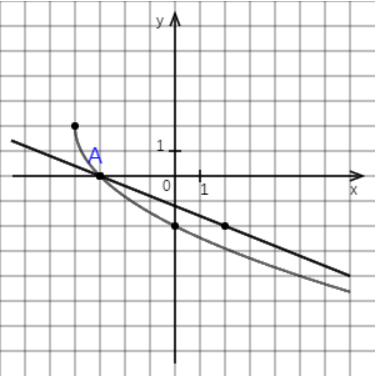
\includegraphics[width=0.45\textwidth]{1}\end{multicols}

\begin{multicols}{2}
	\fbox{\parbox{0.45\textwidth}{
			На рисунке изображены графики функций $f(x)=a\sqrt{x-b}+c$ и $g(x)=kx-d$,
			которые пересекаются в точках A и B. Найдите абсциссу точки B.
			\\\\Решение:\\\\
			$f(x)=2\sqrt{x+5}-5$

			$g(x)=0,5x-2,5$

			$A(-5;-5)$

			$B(11;3)$
		}}

	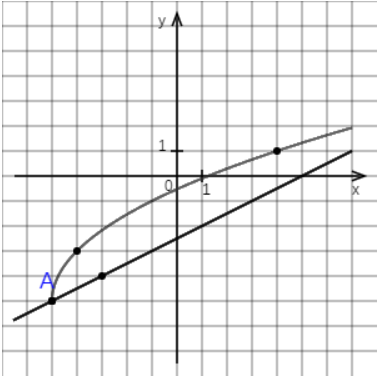
\includegraphics[width=0.45\textwidth]{2}\end{multicols}

\begin{multicols}{2}\fbox{\parbox{0.45\textwidth}{На рисунке изображены графики функций $f(x)=a\sqrt{x-b}+c$ и $g(x)=kx-d$,
			которые пересекаются в точках A и B. Найдите ординату точки B.
			\\\\Решение:\\\\
			$f(x)=2\sqrt{x+0}-3$

			$g(x)=0,5x-1,5$

			$A(1;-1)$

			$B(9;3)$
		}}

	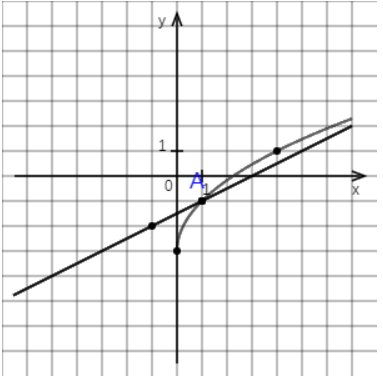
\includegraphics[width=0.45\textwidth]{3}\end{multicols}

%%%%%%%%%%%%%%%%%%%%%


\subsubsection*{Задание №3509123}
\lstinputlisting{code/ex_509123.js}
Примеры генерируемых задач:


\begin{multicols}{2}\fbox{
		\parbox{0.45\textwidth}{На рисунке изображён график функции $f(x)=a \ctg x+b$. Найдите $b$.
			\\\\Решение:\\\\
			$f(x)=2\ctg x-2$}}

	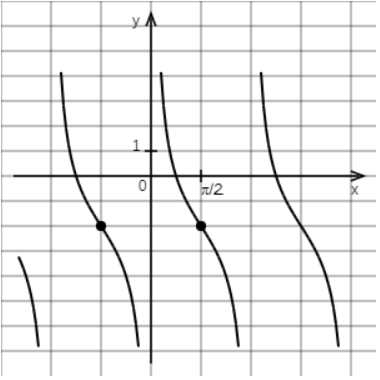
\includegraphics[width=0.45\textwidth]{4}\end{multicols}

\begin{multicols}{2}\fbox{
		\parbox{0.45\textwidth}{
			На рисунке изображён график функции $f(x)=a \cos x+b$. Найдите $a$.
			\\\\Решение:\\\\
			$f(x)=-4\cos x+2$}}

	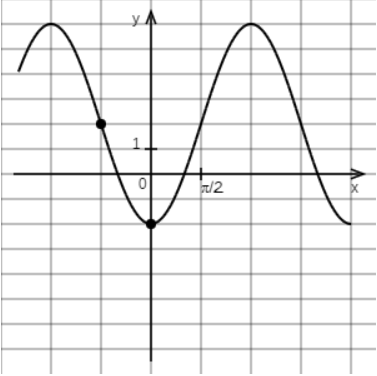
\includegraphics[width=0.45\textwidth]{5}\end{multicols}

\begin{multicols}{2}\fbox{
		\parbox{0.45\textwidth}{
			На рисунке изображён график функции $f(x)=a \sin x+b$. Найдите $b$.
			\\\\Решение:\\\\
			$f(x)=6 \sin x-3$
		}}

	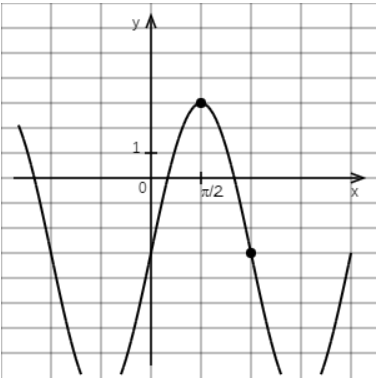
\includegraphics[width=0.45\textwidth]{6}\end{multicols}

\subsubsection*{Задание №317541}
\lstinputlisting{code/ex_317541.js}

Примеры генерируемых задач:

\begin{multicols}{2}\fbox{
		\parbox{0.45\textwidth}{
			На рисунке изображён график дифференцируемой функции $y=f(x)$. На оси абсцисс отмечены 5 точек : $x_1, x_2, x_3, \dots, x_5$. Среди этих точек найдите все точки, в которых производная функции $f(x)$ положительна. В ответе укажите количество найденных точек.
		}}

	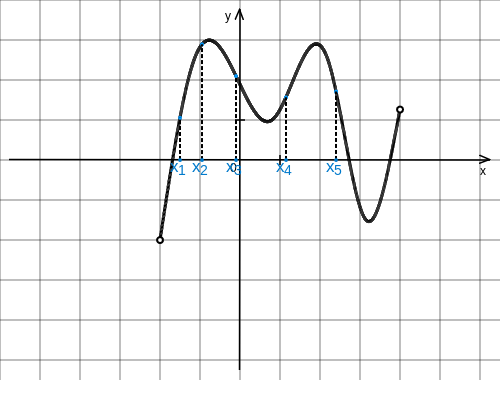
\includegraphics[width=0.45\textwidth]{7}\end{multicols}

\begin{multicols}{2}\fbox{
		\parbox{0.45\textwidth}{
			На рисунке изображён график $y=f'(x)$ — производной функции $f(x)$. На оси абсцисс отмечены 5 точек: $x_1, x_2, x_3, \dots, x_5$. Сколько из этих точек лежит на промежутках возрастания функции $f(x)$?

		}}

	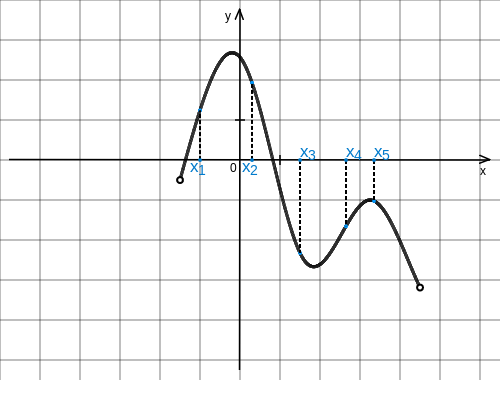
\includegraphics[width=0.45\textwidth]{8}\end{multicols}

\begin{multicols}{2}\fbox{
		\parbox{0.45\textwidth}{
			На рисунке изображён график дифференцируемой функции $y=f(x)$. На оси абсцисс отмечены 5 точек : $x_1, x_2, x_3, \dots, x_5$. Среди этих точек найдите все точки, в которых производная функции $f(x)$ положительна. В ответе укажите количество найденных точек.

		}}

	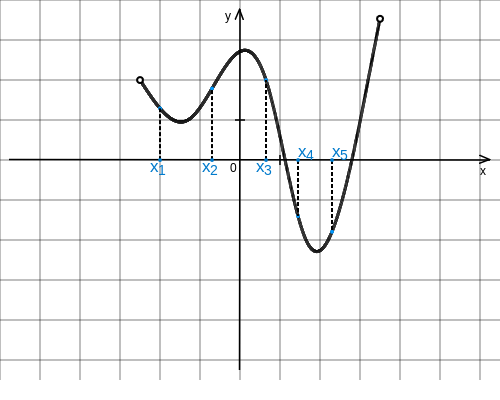
\includegraphics[width=0.45\textwidth]{9}\end{multicols}

\newpage	
\subsubsection*{Задание №317544}
\lstinputlisting{code/ex_317544.js}

	\begin{multicols}{2}\fbox{
		\parbox{0.45\textwidth}{
			На рисунке изображен график функции $y=f(x)$ и отмечены точки $-6,6$; $9,6$; $2,1$; $5$. В какой из этих точек значение производной наибольшая? В ответе укажите эту точку.
		}}

	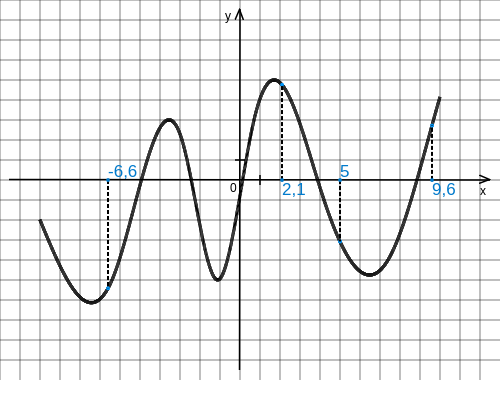
\includegraphics[width=0.45\textwidth]{10}\end{multicols}

\newpage
\begin{multicols}{2}\fbox{
		\parbox{0.45\textwidth}{
			На рисунке изображен график функции $y=f(x)$ и отмечены точки $-9$; $1,7$; $-3,7$; $5,1$. В какой из этих точек значение производной наибольшая? В ответе укажите эту точку. 
		}}

	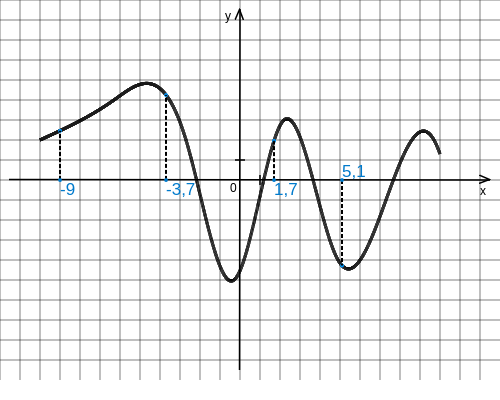
\includegraphics[width=0.45\textwidth]{11}\end{multicols}

\begin{multicols}{2}\fbox{
		\parbox{0.45\textwidth}{
			На рисунке изображен график функции $y=f(x)$ и отмечены точки $5,6$; $-3,1$; $8,6$; $0,7$. В какой из этих точек значение производной наименьшее? В ответе укажите эту точку. 
		}}

	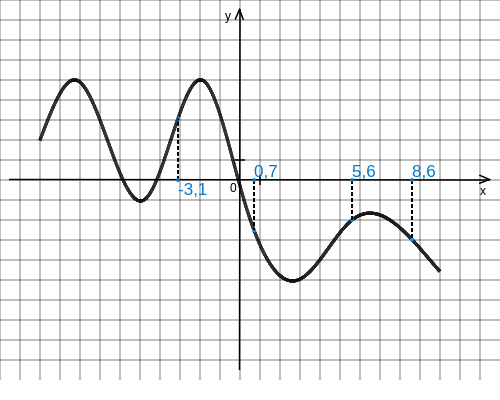
\includegraphics[width=0.45\textwidth]{12}\end{multicols}

\section*{Заключение}
\addcontentsline{toc}{section}{Заключение}
В данной работе были приведены архитектура проекта «Час ЕГЭ», его библиотеки
и примеры генерируемых задач. Обоснована релевантность проекта по сравнению
с другими открытыми ресурсами.

В дальнейшем автор продолжит расширять каталог
заданий по математике (в частности новых заданий номер 7 и 10) и будет способствовать появлению тестов по другим предметам.
%%А также дополнит проект новым лексическим модулем, связанным с изменением
%%глаголов по времени и роду в прошедшем времени.



\begin{thebibliography}{5}
	\bibitem{chasdok1} Момот Е. А., Арахов Н. Д. Разработка и внедрение ПО для сбора статистики результатов подготовки к ЕГЭ по математике профильного уровня //Актуальные проблемы прикладной математики, информатики и механики. – 2021. – С. 1-2.
	\bibitem{egemath}Открытый банк задач ЕГЭ по Математике.Профильный уровень. – URL:  https://prof.mathege.ru/
	\bibitem{chasi}Пошаговая инструкция по созданию элементарных шаблонов. – URL:  https://math.vsu.ru/chas-ege/doc/shabl-b1-po-shagam.html
	\bibitem{fipi}Федеральный институт педагогических измерений. – URL:  https://fipi.ru/ege/otkrytyy-bank-zadaniy-ege
	\bibitem{ege} Единый государственный экзамен. – URL:  https://ru.wikipedia.org/wiki/Единый\_государственный\_экзамен
\end{thebibliography}
\end{document}
